\documentclass{article}

\usepackage{geometry}
\usepackage{hyperref}
\usepackage{graphicx}
\usepackage{afterpage}

\title {Khidmat: Award Management System at DYSF}

\author{
  Sameer Anees Jaliawala\\ sj02732 
}
\date{}  

\begin{document}
\maketitle

% Use first person plural (we, us) even if you did the Khidmat individually.

% An introduction of the project, no more than 2 sentences. Provide the highest level of detail only. Other details will come later.
% Typically, "This project is to <short description of porject> for/at <client>."
This project is to create an Award Management System. Furthermore, we will also be somewhat involved in all other side projects related to IT such as the DYSF Portal and the Scholarship Management System.  

% About the client.
DYSF is a non-profit organization that represents the Dhoraji Memons and the youth of the community. DYSF's mission is to strive for transformation of Dhoraji Memons into a highly educated, self reliant, progressive and healthy community. More On:\newline \href{http://www.dhorajiyouth.org/aboutus.aspx?page=about}{http://www.dhorajiyouth.org/aboutus.aspx?page=about}

% About the project.
DYSF has a an award ceremony every year where hundreds of Dhoraji Memon students from all education background receive awards for their achievements in their studies. However, most of the system relies on manual entry of paper based forms and the use of excel to generate lists which is a highly inefficient system in this technologically advanced era. Our objective is to make an efficient system, that makes use of database technology, which could ease the overall process. Moreover, we would also give our contributions to IT related projects that will be taking place during our khidmat which are: The DYSF Portal and the DYSF Scholarship Management System. All the work will be done by the DYSF IT Team, which includes us.

% About the plan of work.
We will work part time for DYSF under the supervision of their IT supervisor, who is one of their board of governors. Our main work would take place at our own convenient time and place and their is no particular deadline set for the project. The goal is to develop, test, and deploy the award management system by the end of our Khidmat.

% Copy-paste this section with necessary modifcations for each week.
\newpage % Start the report for each week on a new page.
\section*{Week 1: 27 May -- 2 June, 2018}

% A summary, maximum 2 sentences, of this week's activities.
We spent this week meeting the IT team we would work with. We laid down objectives and aims and also decided on the division of labour. We checked out the annual award's current manual system, as well as the inoperative DYSF scholarship system at the DYSF office. We also paid a visit to Expertek Solutions, the firm which handled all their IT business and also made their website. \newline

\begin{tabular}{|l|l|l|l|}
  \hline
  Item 	& Activity & Time & ID \\\hline\hline
  1	& Met IT team and supervisor & 2 hrs & sj02732 \\\hline
  2	& Checked out the current IT system at DYSF office & 2 hrs & sj02732 \\\hline
  3	& Meeting at Expertek Solutions & 2 hrs & sj02732 \\\hline
  4 & Research, Brainstorming, Learning html,css,php & 1hr and 30mins & sj02732  \\\hline
\end{tabular}
\newline
The total time spent on the Khidmat this week is as follows.

\begin{tabular}{|l|l|}
  \hline
  ID & Total Hours\\\hline\hline
  sj02732 & 7 hours and 30 mins\\\hline
\end{tabular}

% Other weeks ...
\newpage % Start the report for each week on a new page.
\section*{Week 2: 3--9 June, 2018}

% A summary, maximum 2 sentences, of this week's activities.
Meeting with the external supervisor. He wanted to know what we thought of the current award system and how we can improve it. We told him about our ideas and how we can make the system better. We also explained the problems about the scholarship system. We made a draft ERD of the award system. The IT team met together to bring up a lsit of problems and objectives. \newline

\begin{tabular}{|l|l|l|l|}
  \hline
  Item 	& Activity & Time & ID \\\hline\hline
  1	& Met IT team and supervisor & 2 hrs & sj02732 \\\hline
  2	& Making draft ERD and learning php,html,css & 3 hrs & sj02732 \\\hline
  3	& 1st kickstart meeting with IT team & 2 hrs & sj02732 \\\hline
\end{tabular}
\newline
The total time spent on the Khidmat this week is as follows.

\begin{tabular}{|l|l|}
  \hline
  ID & Total Hours\\\hline\hline
  sj02732 & 7 hrs\\\hline
\end{tabular}

\newpage % Start the report for each week on a new page.
\section*{Week 3: 10--16 June, 2018}

% A summary, maximum 2 sentences, of this week's activities.
Created database on the base of the draft ERD made last week. We also made ourselves aware of PHP myadmin and its database operations. We made our own effort on the user end forms. We divivded the forms into 4 parts and worked on the first part. \newline

\begin{tabular}{|l|l|l|l|}
  \hline
  Item 	& Activity & Time & ID \\\hline\hline
  1	& Created Database on PHP myadmin & 3 hrs & sj02732 \\\hline
  2	& Made user-end form on html and linked it with database(PHP) & 3 hrs & sj02732 \\\hline
\end{tabular}
\newline
The total time spent on the Khidmat this week is as follows.

\begin{tabular}{|l|l|}
  \hline
  ID & Total Hours\\\hline\hline
  sj02732 & 6 hrs\\\hline
\end{tabular}

\newpage % Start the report for each week on a new page.
\section*{Week 4: 17--23 June, 2018}

% A summary, maximum 2 sentences, of this week's activities.
We made 2 more user-end forms out of the 4 forms. We added validation checks and added final queries to them.  \newline

\begin{tabular}{|l|l|l|l|}
  \hline
  Item 	& Activity & Time & ID \\\hline\hline
  1	& Made 2 more user-end forms on html & 3-4 hrs & sj02732 \\\hline
  2	& Added sql queries and validation checks. Testing and debugging. & 3-4 hrs & sj02732 \\\hline
\end{tabular}
\newline
The total time spent on the Khidmat this week is as follows.

\begin{tabular}{|l|l|}
  \hline
  ID & Total Hours\\\hline\hline
  sj02732 & 7 hrs\\\hline
\end{tabular}

\newpage % Start the report for each week on a new page.
\section*{Week 5: 24--30 June, 2018}

% A summary, maximum 2 sentences, of this week's activities.
Meeting with the external supervisor. We updated him about our work. The IT team told us to leave the user-end for now and to focus on the admin-end of the system. We decided we would work on Laravel and use AdminLTE as the template. We also had an internal meeting with the IT team. (This was the first time we met after Eid) \newline

\begin{tabular}{|l|l|l|l|}
  \hline
  Item 	& Activity & Time & ID \\\hline\hline
  1	& Met IT team and supervisor & 2 hrs & sj02732 \\\hline
  2	& 2nd kickstart meeting with IT team & 2 hrs & sj02732 \\\hline
  3	& Researched Laravel and implemented AdminLTe on our systems & 3 hrs & sj02732 \\\hline
\end{tabular}
\newline
The total time spent on the Khidmat this week is as follows.

\begin{tabular}{|l|l|}
  \hline
  ID & Total Hours\\\hline\hline
  sj02732 & 7 hrs\\\hline
\end{tabular}

\newpage % Start the report for each week on a new page.
\section*{Week 6: 1--7 July, 2018}

% A summary, maximum 2 sentences, of this week's activities.
Our IT Team head advised us to use Stack template instead as it had better security. We went ahead and implemented on our system. We brainstormed how the system would look like on the template and also brought up some ideas on the dashboard. We started making the first CRUD on the system ( the CRUD related to the table known as Awardees). \newline

\begin{tabular}{|l|l|l|l|}
  \hline
  Item 	& Activity & Time & ID \\\hline\hline
  1	& Implemeted and brainstormed on Stack template and its usage & 2 hrs & sj02732 \\\hline
  2	& Started making the first CRUD of the system & 3 hrs & sj02732 \\\hline
\end{tabular}
\newline
The total time spent on the Khidmat this week is as follows.

\begin{tabular}{|l|l|}
  \hline
  ID & Total Hours\\\hline\hline
  sj02732 & 5 hrs\\\hline
\end{tabular}

\newpage % Start the report for each week on a new page.
\section*{Week 7: 8--14 July, 2018}

% A summary, maximum 2 sentences, of this week's activities.
Met with the external supervisor and IT team (joint meeting) to discuss about all the IT projects in development. Met exclusively with external supervisor and IT head to find any other features in the system and how they want the data to be organized. We also finsished making the first CRUD of the system and started on the second CRUD(Degrees). \newline

\begin{tabular}{|l|l|l|l|}
  \hline
  Item 	& Activity & Time & ID \\\hline\hline
  1	& Meeting with external supervisor and IT team & 2 hrs & sj02732 \\\hline
  2	& Second Meeting with external supervisor and IT head & 2 hrs & sj02732 \\\hline
  3	& Started making the second CRUD and finished on the first CRUD & 2 hrs & sj02732 \\\hline
\end{tabular}
\newline
The total time spent on the Khidmat this week is as follows.

\begin{tabular}{|l|l|}
  \hline
  ID & Total Hours\\\hline\hline
  sj02732 & 6 hrs\\\hline
\end{tabular}

\newpage % Start the report for each week on a new page.
\section*{Week 8: 15--21 July, 2018}

% A summary, maximum 2 sentences, of this week's activities.
We met with the IT team head this week, who helped us alot on the application. We finished our second and third CRUD (Majors) this week and started working on implementing the 4th Crud(Family History) and merging it with 1st CRUD (Members). \newline

\begin{tabular}{|l|l|l|l|}
  \hline
  Item 	& Activity & Time & ID \\\hline\hline
  1	& Meeting with IT team head & 2 hrs & sj02732 \\\hline
  2	& Finished making the second and third CRUD  & 3 hrs & sj02732 \\\hline
  3	& Started implementing the fourth Crud and merging it with first Crud & 1 hrs & sj02732 \\\hline
\end{tabular}
\newline
The total time spent on the Khidmat this week is as follows.

\begin{tabular}{|l|l|}
  \hline
  ID & Total Hours\\\hline\hline
  sj02732 & 6 hrs\\\hline
\end{tabular}

\newpage % Start the report for each week on a new page.
\section*{Week 9: 22--28 July, 2018}

% A summary, maximum 2 sentences, of this week's activities.
The IT team head checked our progress and also helped us in our application. (We are meeting with the IT team head weekly). We merged the 4th CRUD with the 1st CRUD (which is difficult to do in Laravel). We also made Calender Cards on the dashboard( these cards let the user know days left to certain events). We started working on the seating arrangement feature of the application. \newline

\begin{tabular}{|l|l|l|l|}
  \hline
  Item 	& Activity & Time & ID \\\hline\hline
  1	& Meeting with IT team head & 1.30 hrs & sj02732 \\\hline
  2	& Merged and implemented the 4th CRUD with the 1st CRUD. & 2 hrs & sj02732 \\\hline
  3	& Made Calender Cards on Dashboard & 1 hrs & sj02732 \\\hline
  4	& Started working on the seating arrangement feature  & 1 hrs & sj02732 \\\hline
\end{tabular}
\newline
The total time spent on the Khidmat this week is as follows.

\begin{tabular}{|l|l|}
  \hline
  ID & Total Hours\\\hline\hline
  sj02732 & 5.30 hrs\\\hline
\end{tabular}

\newpage % Start the report for each week on a new page.
\section*{Week 10: 29 July -- 5 August, 2018}

% A summary, maximum 2 sentences, of this week's activities.
Weekly meeting with the IT team head. We completed making the seating arrangement feature which was to generate seat numbers to applicants according to their gender and award categories(Degree) and listed them in a proper format. We made the layout of the seating tickets which the user can print once all the seats are generated. We also made interactive charts on the dashboard that show graphical representation of data.   \newline

\begin{tabular}{|l|l|l|l|}
  \hline
  Item 	& Activity & Time & ID \\\hline\hline
  1	& Weekly Meeting with IT team head & 1.30 hrs & sj02732 \\\hline
  2	& Completed making the seating arrangement feature(including tickets)  & 4 hrs & sj02732 \\\hline
  3	& Made charts on the Dashboard & 2 hrs & sj02732 \\\hline
\end{tabular}
\newline
The total time spent on the Khidmat this week is as follows.

\begin{tabular}{|l|l|}
  \hline
  ID & Total Hours\\\hline\hline
  sj02732 & 7.30 hrs\\\hline
\end{tabular}

\newpage
\section*{Conclusion}

% Remind the reader about the project. Summarise your activities over the course of the project.
Our project was to build an Award Management System for Dhoraji Youth Service Foundation. We started by meeting the external supervisor and IT team to discuss how to build this system. Initially, we decided to make both the user-end and admin-end of the system. However, due to some reasons our IT team advised us to only focus on the admin-end. We then identified the necessary tools to build the required system and trained ourselves on them. The system was built on PHP Laravel using Eloquent ORM to work with our Database. Development and testing were carried out in collaboration with the IT team head so that any shortcomings were identified and catered to as we went along. After development, we gave the system to the IT team head and also gave the demo to the external supervisor and all those involved from the administration. The deployment responsibility has been undertaken by the IT team head and the external supervisor; as they ensured us that they are going to deploy the system as soon as they get the hosting for it. We also attended meetings and gave a hand in other IT projects that were going on during our time there.


\newpage
% Show your external supervisor your report, especially the weekly upates; have them sign a printed copy of this page; scan the signed page; and include the scanned page in this document as an image.

% Insert your name below.
\afterpage{%
\newgeometry{top=0cm,bottom=0cm,left=0cm,right=0cm,nohead,nofoot}
% material for this page
\begin{figure}
  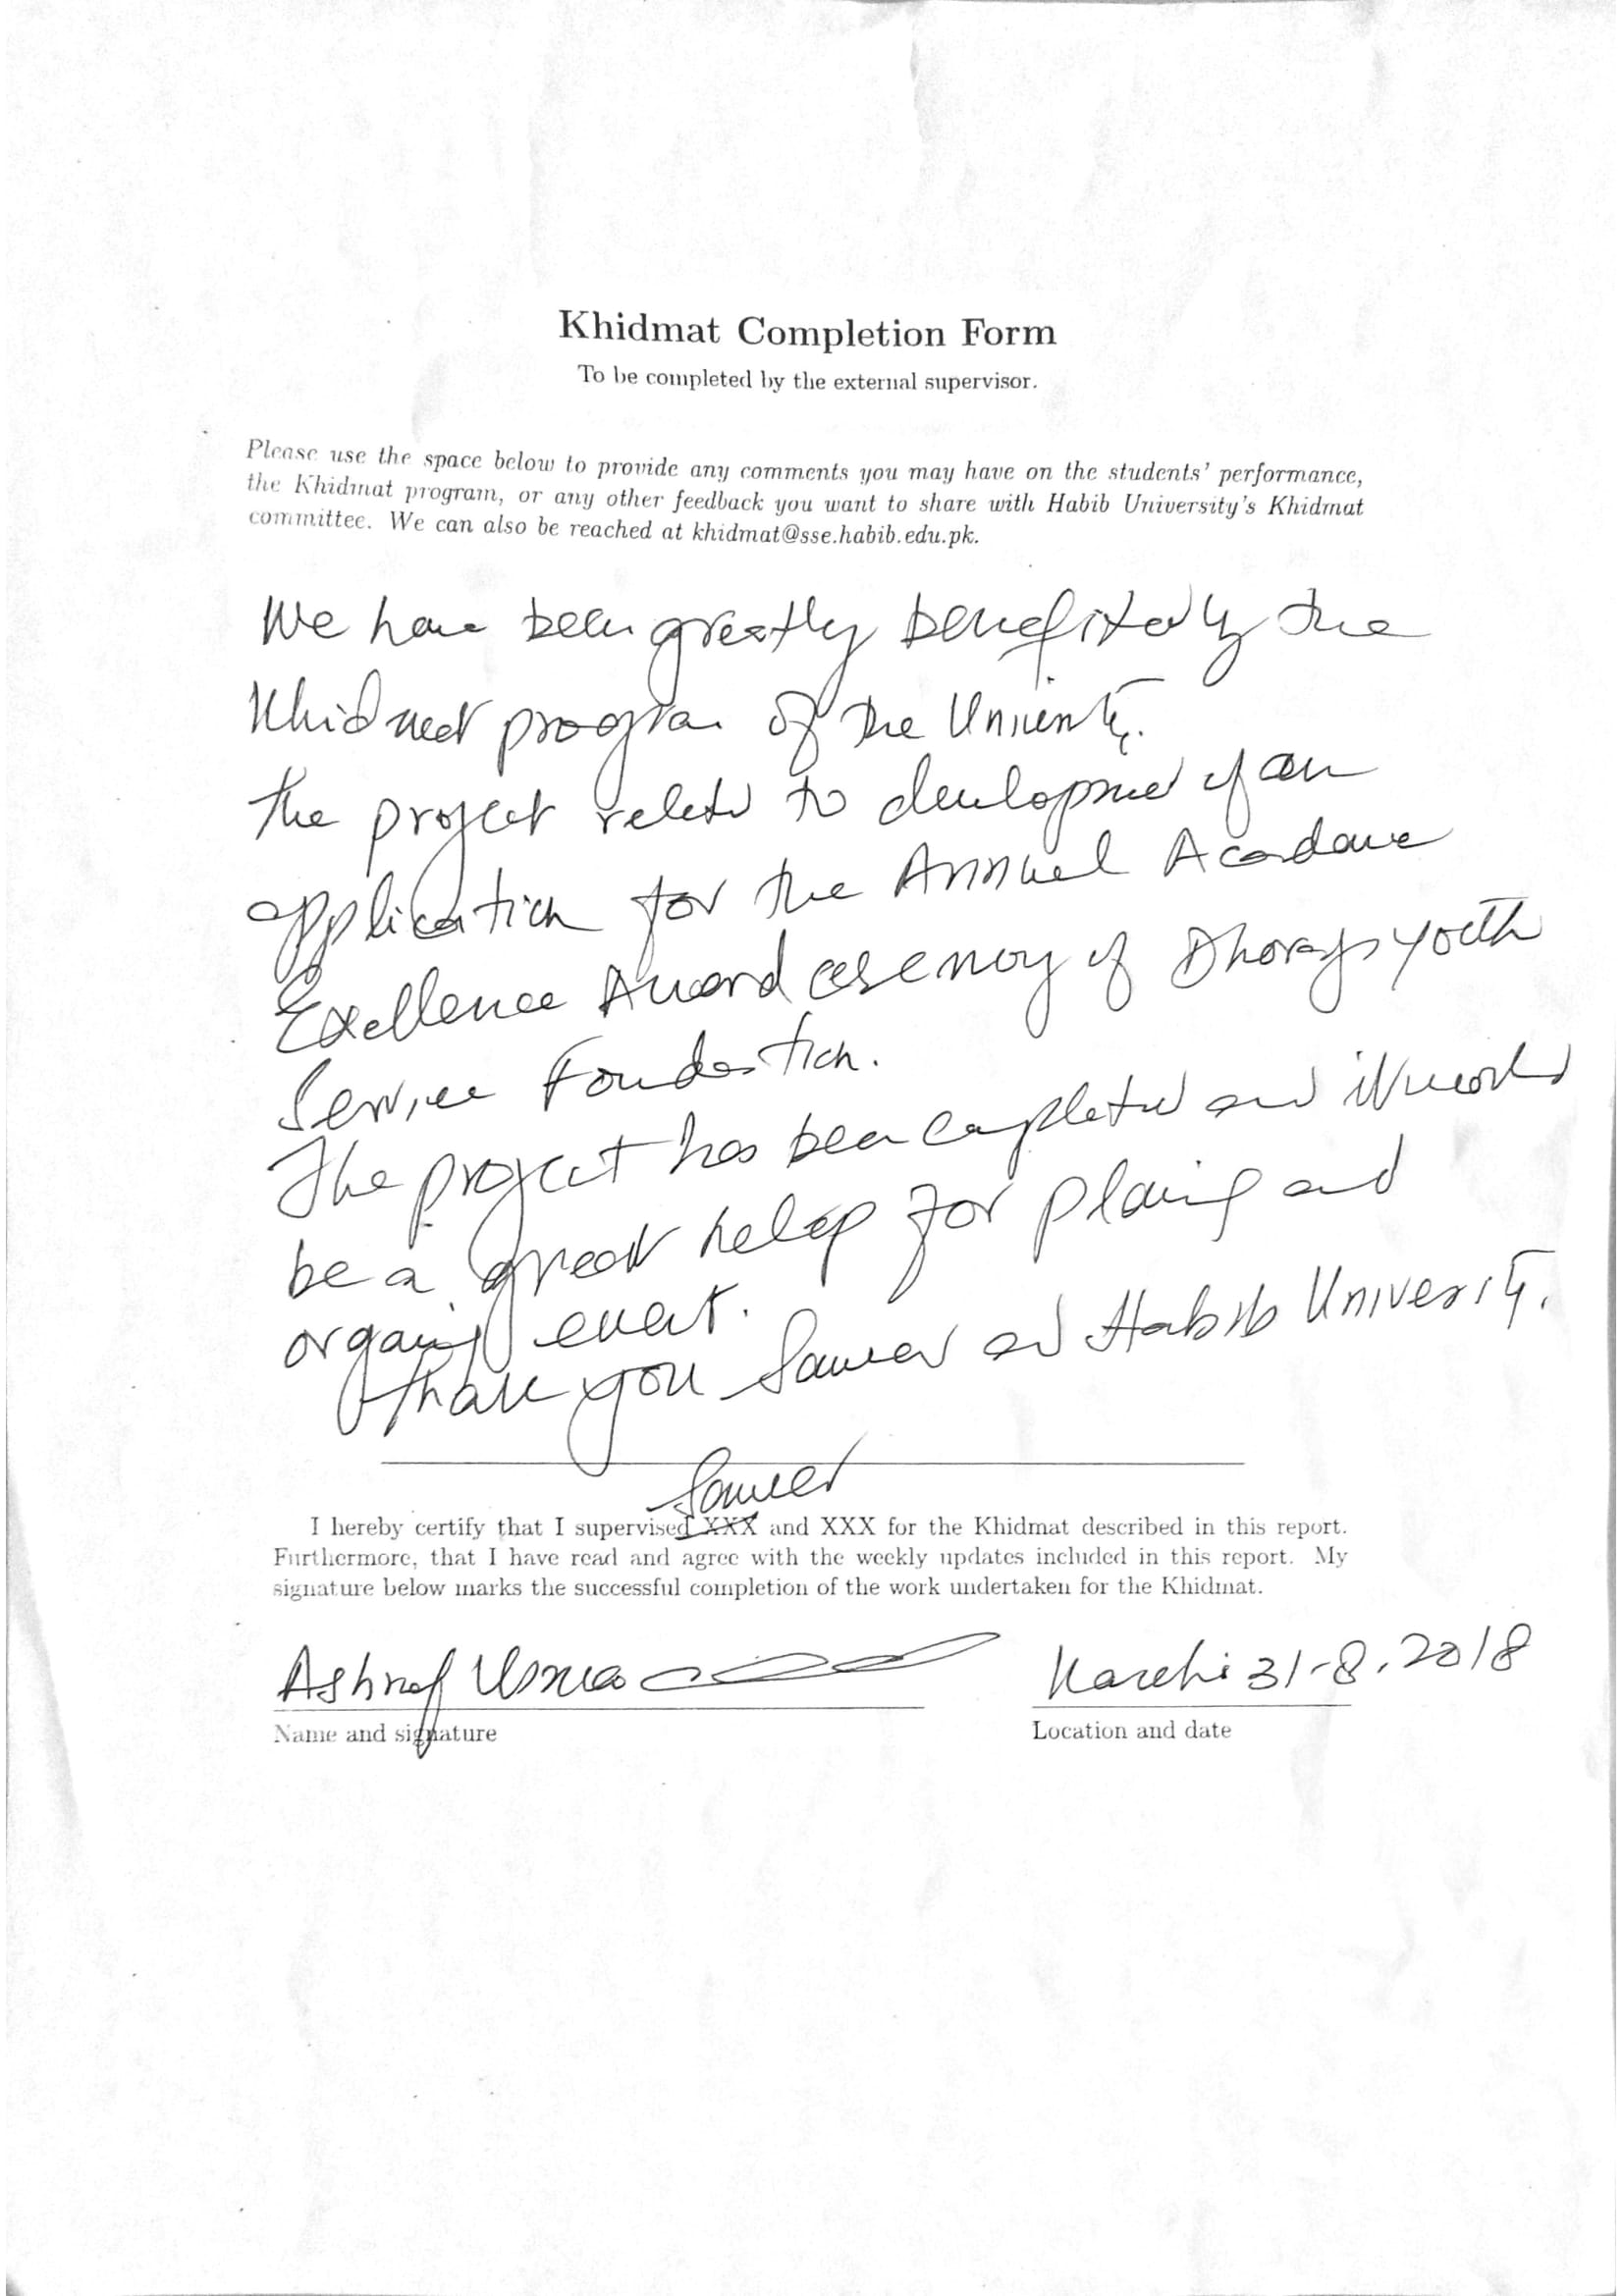
\includegraphics[width=0.97\textwidth]{last_page.jpg}
\end{figure}

\clearpage
\restoregeometry
}
\end{document}
